\documentclass[12pt,reqno]{amsart}
\usepackage{amsfonts,amssymb,amsmath,amsthm,
            amssymb,amsopn,amsxtra,amstext,amsbsy}
\usepackage{epsfig}
\usepackage[makeroom]{cancel}
\usepackage{array,arydshln}
\usepackage{array}
\usepackage{url}
%\usepackage{tikz}
\usepackage[spanish]{babel}
\usepackage[utf8x]{inputenc}
\usepackage{fancyhdr}
\usepackage{graphicx}
\usepackage{hyperref,wasysym}
\usepackage{color}
\usepackage{enumerate}
\usepackage{algorithm}
\usepackage{algorithmic}
\renewcommand{\algorithmicrequire}{\textbf{Input:}}
\renewcommand{\algorithmicensure}{\textbf{Output:}}

\newtheorem*{myteo}{Teorema}
\newtheorem*{mydef}{Definici\'on}

\voffset=-10mm
\oddsidemargin=0pt
\evensidemargin=0pt
\topmargin=-10mm
\headsep=10mm
\headheight=18pt
\footskip=30pt
\topskip=0mm
\textwidth 167mm
\textheight=230mm
\parindent=5mm
\marginparsep=3mm
\marginparwidth=19mm
\vfuzz2pt % Don't report over-full v-boxes if over-edge is small
\hfuzz6pt % Don't report over-full h-boxes if over-edge is small


%% MYREMARK ENVIRONMENT %%%%%%%%%%%
\newenvironment{mycolor}{\color{red}}{}
\newcounter{myremarkcount}
\setcounter{myremarkcount}{0}
\newsavebox{\myremarkbox}
\newenvironment{myremark}
{% This is the begin code
\medskip
\begin{flushright}
\begin{lrbox}{\myremarkbox}%
\begin{minipage}[t]{0.9\linewidth}
\stepcounter{myremarkcount}
\footnotesize
\begin{mycolor}
{\bf Remark \arabic{myremarkcount}.}
\begin{it}
}
{% This is the end code
\end{it}
\end{mycolor}
\end{minipage}
\end{lrbox}
\fbox{\usebox{\myremarkbox}}
\end{flushright}

\bigskip}


\title{A Time Varying Vector Error Correction Model Applied to Foreign Exchange
Market}
\author{Paola Arce \and Jonathan Antognini \and Luis Salinas \and Werner Kristjanpoller}


\begin{document}
\maketitle

\begin{abstract}
Financial time series are known for their non-stationary behaviour. However,
sometimes they exhibit some stationary linear combinations. When this happens,
it is said that those time series are cointegrated. Vector error correction
model (VECM) is an econometric model which characterizes the joint dynamic
behaviour of a set of cointegrated variables in terms of forces pulling towards
equilibrium. 

VECM parameters are obtained using the ordinary least squares (OLS)
method.  Even though OLS is extensively used, it has over-fitting
issues and is computationally expensive. Ridge regression is commonly used
instead of OLS since they include a regularization parameter which could improve
prediction error.

In this study, we propose an online VECM which optimizes how model parameters
are obtained by using only relevant past data and RR instead of OLS.  Our
proposal also takes advantage of the long-run relationship between the time
series in order to obtain improved execution times. Our proposed method is
tested using synthetic data and foreign exchange rates.
Results show that our proposal enables execution time to be reduced by at least
50\% while maintaining good accuracy levels.
\end{abstract}



\section{Introduction}
The learning from examples problem is an ill-posed problem which
admits an infinite number of solutions.  In order to restrict the
space of admissible solutions, the regression problem is usually
formulated in terms of regularization theory~\cite{girosiETal1995} as
an optimization problem, which minimizes the functional: 

\begin{equation}
\label{eq:problem} 
J(\mathbf{w}) = \sum_{t=1}^m (y_t - f(\mathbf{x}_t))^2 + \gamma R(\mathbf{w})
, \qquad f \in \mathcal{H} \, ,
\end{equation}

\noindent where $m$ is the number of samples $(\mathbf{x}_t ,y_t)$ with
$\mathbf{x}_t \in \R^l$, $l$ correspond to the number of features, $y_t
\in \R$ is the target, $R(\mathbf{w}) = ||w||^2$ where $||.||^2_K$ is a norm in a
{\em reproducing kernel hilbert space} $\mathcal{H}$ defined by the
positive definite form $K$, and $\gamma$ is a regularization
parameter~\cite{evgeniouETal2000}.
%Qué norma debe usarse? falta definir K
When the hypothesis space is reduced, the risk of overfitting the training data
decreases and therefore leading to better generalization capability. 
%aclarar porqué se reduce el espacio de hipótesis
{\em Ridge regression} (RR) is a batch method generally used to solve this
problem, which is a generalization of least squares method (LS). 

%RR is a batch method and it is not used in an online context mainly because
%it uses large amount of data and the number of operations increases
%with data size.

However, online algorithms are more attractive than batch algorithms because
their simplicity and ability to manage large data sets, this is why
they are popular in financial applications.

There are several popular online methods such as
perceptron~\cite{rosenblatt58},
passive-aggressive~\cite{crammerETall2006}, stochastic gradient
descent~\cite{zhang2004}, aggregating algorithm~\cite{vovk2001} and
the second order perceptron~\cite{cesa-bianchi2005}.
In~\cite{cesa-bianchi2006} it is provided an in-deph analysis of
online learning.

The {\em aggregating algorithm for regression} (AAR) method formulates
a recursive formulation of RR in an online way. AAR
consider all data to make a prediction, but in highly variant
scenarios the old data could be useless.

In this paper, we propose an online method based on the idea presented
by~\cite{vovk2001} considering in our case a single sliding window of
the most recent data. This proposal also reduces the number of
operations at every step of the algorithm by expressing the inverse
matrix in an iterative form. Our algorithm is later tested with
financial data from stock market.



\section{Background}
\label{sec:background}

\subsection{Integration and Cointegration}\label{sec:coint}\  
Following \cite{johansen1995} we shall say that a stochastic process
$Y_t$ which satisfies $Y_t-E(Y_t) = \sum_{i=0}^\infty C_i\,\varepsilon_{t-i}$ is
called $I(0)$, and then we shall write $Y_t\sim I(0)$, whenever
$\sum_{i=0}^\infty C_i \neq 0$ and $\sum_{i=0}^\infty C_i\,z^i$ converges for
$z\in\mathbb{C}$ with $|z|<1$.  It is understood that the condition
$\varepsilon_t\sim iid(0,\sigma^2)$ holds.

A (vector) time series $\mathbf{y}_t$ is said to be {\em integrated of order\/}
$d$, and then we shall write $\mathbf{y}_t\sim I(d)$, whenever after $d$ times
(discrete) differentiation an stationary process is
obtained, see \cite{banerjee1993}; more precisely, whenever
$(1-L)^d\,\mathbf{y}_t\sim\text{I(0)}$, where $L$ is the usual lag operator:
$(1-L)\,\mathbf{y}_t = \Delta\mathbf{y}_t = \mathbf{y}_t-\mathbf{y}_{t-1}$ for
all $t$.  

Note that this definition includes the scalar case as time series of vectors of
dimension 1; in this scalar case we will write the time series in nonbold
format.

Let $\mathbf{y}_t^\nu$, $\nu=1,\dots,l$, be a set of $l$ vector time series of
order $I(1)$.  They are said to be {\em cointegrated\/} if a vector
$\beta=[\beta(1),\dots,\beta(l)]^\top \in \mathbb{R}^p$ exists, such that the
time series,
\begin{equation}
\mathbf{Z}_t:= 
\sum_{\nu=1}^l \beta(\nu)\,\mathbf{y}_t^\nu\,\sim\,\text{I(0)}\,.
\end{equation}
In other words, a set of $I(1)$ time series is said to be cointegrated if a
linear combination of them exists, which is I(0).


\subsection{Vector Autorregresive Models}\label{sec:varvec}

Vector error correction model (VECM) describe the joint behaviour of a set of
variables and can be derived from the simple Vector Autoregressive model (VAR)
presented by \cite{sims1980}.  The VAR($p$) model is a framework describing the
behaviour of a set of $l$ endogenous and stationary variables as a linear
combination of their last $p$ values, where $l,p\in\mathbb{N}$.  In our case,
each one of these $l$ variables is a scalar time series $y_{\lambda,t}$,
$\lambda=1,\dots,l$, and we represent them all together at time $t$ by the
vector time series:
\begin{equation}
\label{eq:variables}
\mathbf{y}_t = 
\begin{bmatrix} y_{1,t} & y_{2,t} & \dots & y_{l,t} \end{bmatrix}^\top.
\end{equation}
\noindent
Notice that the vectors $\mathbf{y}_t$ are assumed to be $l$-dimensional.

The VAR($p$) model describes the behaviour of a dependent variable in terms of
its own lagged values and the lags of the others variables in the system. The
model with $p$ lags is formulated as the system:
\begin{align}
\label{eq:var}
\mathbf{y}_t 
= \boldsymbol{\Phi}_1 \mathbf{y}_{t-1} +
  \boldsymbol{\Phi}_2 \mathbf{y}_{t-2} + \dots +
  \boldsymbol{\Phi}_p\mathbf{y}_{t-p} +
  \mathbf{c} + \boldsymbol{\epsilon}_t \nonumber \\
t=p+1,\dots,N,
\end{align}
\noindent where 
$\boldsymbol{\Phi}_1, \boldsymbol{\Phi}_2,\dots,\boldsymbol{\Phi}_p$
are $l\times l$-matrices of real coefficients,
$\boldsymbol{\epsilon}_{p+1},
 \boldsymbol{\epsilon}_{p+2}, \dots, \boldsymbol{\epsilon}_N$ 
are error terms, $\mathbf{c}$ is a constant vector and $N$ is the total
number of samples.

Notice that, regarding our notation of section (\ref{sec:coint}),
we have here 
$\mathbf{y}_t^0 = \mathbf{y}_t$,
$\mathbf{y}_t^\nu = \mathbf{y}_{t-\nu}$ and
the $\lambda$-th component of the vector time series $\mathbf{y}_t^\nu$
is the scalar time series $y_{\lambda,t}^\nu$, where $\nu=1,\dots,p$ and
$\lambda=1,\dots,l$.

However, the VAR model cannot be used with non-stationary variables. VECM ,
developed by \cite{engle87}, is also a linear model for I(1) variables that are
also cointegrated, see \cite{banerjee1993}. If cointegration exists, variable
differences are stationary and they introduce an error correction term which
adjusts coefficients to bring the variables back to equilibrium. 


It is obtained re-writing equation (\ref{eq:var}) in terms of the new
variable $\Delta\mathbf{y}_t=\mathbf{y}_t-\mathbf{y}_{t-1}$.
The VECM model, expressed in terms those differences, takes the form:
\begin{equation}\label{eq:vec}
\Delta \mathbf{y}_t 
= \boldsymbol{\Omega}\,\mathbf{y}_{t-1}
  + \sum_{i=1}^{p-1} \boldsymbol{\Phi}_i^*\,\Delta\mathbf{y}_{t-i}
  + \mathbf{c} + \boldsymbol{\epsilon}_t\,,
\end{equation}
\noindent
where the coefficients matrices $\boldsymbol{\Phi}_i^*$ and 
$\boldsymbol{\Omega}$, expressed in terms of the matrices
$\boldsymbol{\Phi}_i$ of (\ref{eq:var}), are:
\begin{align*}
\boldsymbol{\Phi}_i^* 
&:= -\sum_{j=i+1}^{p}\boldsymbol{\Phi}_j\,, \\
\boldsymbol{\Omega}
&:= -\left( \mathbb{I} - \boldsymbol{\Phi}_1 - \dots 
    - \boldsymbol{\phi}_p \right)\,. 
\end{align*}
The following well known properties of the matrix $\boldsymbol{\Omega}$, see
\cite{johansen1995}, will be useful in the sequel:
\begin{itemize}
\item
If $\boldsymbol{\Omega} = \mathbf{0}$, there is no cointegration.
\item 
If $rank(\boldsymbol{\Omega})=l$, i.e., if $\boldsymbol{\Omega}$ has
full rank, then the time series are not I(1) but stationary.
\item
If $rank(\boldsymbol{\Omega})=r$, $0<r<l$, then there is cointegration
and the matrix $\boldsymbol{\Omega}$ can be expressed as
$\boldsymbol{\Omega}=\boldsymbol{\alpha\beta}^\top$, where $\boldsymbol{\alpha}$
and $\boldsymbol{\beta}$ are
$l\times r$ matrices and
$\text{rank}(\boldsymbol{\alpha})=\text{rank}(\boldsymbol{\beta})=r$.
\item
The columns of $\boldsymbol{\beta}$ contains the cointegration vectors and the rows of
$\boldsymbol{\alpha}$ correspond with the adjusted vectors. 
$\boldsymbol{\beta}$ is obtained by Johansen procedure,see \cite{johansen1988},
whereas $\boldsymbol{\alpha}$ has to be determined as a variable in the VECM.
\end{itemize}
It is worth noticing that the factorization of the matrix
$\boldsymbol\Omega$ is not unique, since for any $r \times r$
non-singular matrix $\mathbf{H}$, $\boldsymbol{\alpha}^*:=\boldsymbol{\alpha}\mathbf{H}$,
and $\boldsymbol{\beta}^*=\boldsymbol{\beta}(\mathbf{H}^{-1})^\top$ we have
$\boldsymbol{\alpha\beta}^\top=\boldsymbol{\alpha}^*(\boldsymbol{\beta}^*)^\top$.
If cointegration exists, then equation (\ref{eq:vec}) can be written
as follows:
\begin{equation}\label{eq:vecfull}
\Delta\mathbf{y}_t 
= \boldsymbol{\alpha\beta}^\top\mathbf{y}_{t-1} 
  + \sum_{i=1}^{p-1}\boldsymbol{\Phi}_i^*\,\Delta\mathbf{y}_{t-i}
  + \mathbf{c} + \boldsymbol{\epsilon}_t\,,
\end{equation}
\noindent
which is a VAR model but for time series differences.


Transposing each equation of the system (\ref{eq:vecfull}) we can write
the VECM($p$) model in block-matrix form as:
\begin{equation}\label{eq:vareq}
\mathbf{B} = 
\mathbf{A} \mathbf{X} + 
\mathbf{E} \, , 
\end{equation}
%
\noindent where $\mathbf{B}$ dimension is $((N-p)\times l)$, $\mathbf{A}$
dimension is $((N-p)\times(r+(p-1)l +1))$, $\mathbf{X}$ dimension is $((r+(p-1)l
+1)\times l)$ and $\mathbf{E}$ dimension is $((N-p)\times l)$:
%
\begin{alignat}{3}
\mathbf{B}
&= \begin{bmatrix}
   \Delta\mathbf{y}_{p+1}^\top \\
   \Delta\mathbf{y}_{p+2}^\top \\
   \vdots \\
   \Delta\mathbf{y}_N^\top
   \end{bmatrix}
&\quad
\mathbf{X}
&= \begin{bmatrix}
   \boldsymbol{\alpha}^\top \\
   \boldsymbol{\Phi}_1^{*\top} \\
   \boldsymbol{\Phi}_2^{*\top} \\
   \vdots \\
   \boldsymbol{\Phi}_{p-1}^{*\top} \\
   \mathbf{c}^\top
   \end{bmatrix}
&\quad
\mathbf{E}
&= \begin{bmatrix}
   \boldsymbol{\epsilon}_{p+1}^\top \\
   \boldsymbol{\epsilon}_{p+2}^\top \\
   \vdots \\
   \boldsymbol{\epsilon}_N^\top \\
   \end{bmatrix}
\end{alignat}
\noindent and 
\begin{align}
\mathbf{A} 
&= \begin{pmat}[{....|}]
   \mathbf{y}_p^\top \boldsymbol{\beta} & \Delta \mathbf{y}_p^\top & \Delta\mathbf{y}_{p-1}^\top & \dots 
                    & \Delta\mathbf{y}_2^\top & 1 \cr
   \mathbf{y}_{p+1}^\top  \boldsymbol{\beta} &\Delta\mathbf{y}_{p+1}^\top & \Delta\mathbf{y}_p^\top & \dots
                       & \Delta\mathbf{y}_3^\top & 1 \cr
   \vdots & \vdots & \vdots & \ddots & \vdots & \vdots \cr
   \mathbf{y}_{N-1}^\top  \boldsymbol{\beta} &\Delta\mathbf{y}_{N-1}^\top & \Delta\mathbf{y}_{N-2}^\top & \dots 
                       & \Delta\mathbf{y}_{N-p-1}^\top & 1 \cr
   \end{pmat}\, .
\label{eq:Amatrix}
\end{align}
Taking into account the error term $\mathbf{E}$, equation~(\ref{eq:vareq}) 
can be solved with respect to $\mathbf{X}$ using the OLS estimation.

\section{Methodology} \label{sec:methodology}
\subsection{Motivation} \label{sec:proposal}

Cointegration vectors can be found applying the Johansen method which uses a
sample of the last historical data. However, VECM assumes cointegration vectors
do not change in time.  In fact, \cite{gregoryETal1996} addresses that the
long-run relationships between the time series  might change due to several
economic factors that can lead to structural breaks in the cointegration
relationship.  In order to show that the number of cointegration vectors depends
on the amount $L$ of historical data and the number of lags $p$ in the VECM, we
used a grid search.  We defined a grid of possible values for $L$ and $p$. $L$
goes throughout $[2,14]$ hours (1 $hour = 360$ data points) with a step size of
4 hours and $p$ throughout $[1,5]$ with step size of 1. The first experiment
consisted in determining the number of cointegration vectors for all
combinations of $L$ and $p$.  We used four forex rates: EURUSD, GBPUSD, USDCHF
and USDJPY with 10-second frequency. Data started at 13:00 GMT of the 13th of
August 2014, when the New York and London financial markets opened.

Figure \ref{fig:hists} shows the distribution of the number of cointegration
vectors given by the Johansen method for different values of $L=[2,6,10,14]$
hours  and $p=1$ . This procedure was carried out by a sliding window of
historical data moving 1000 times.



\begin{figure}[!h]
  %\vspace{-0.8cm}
  \centering
  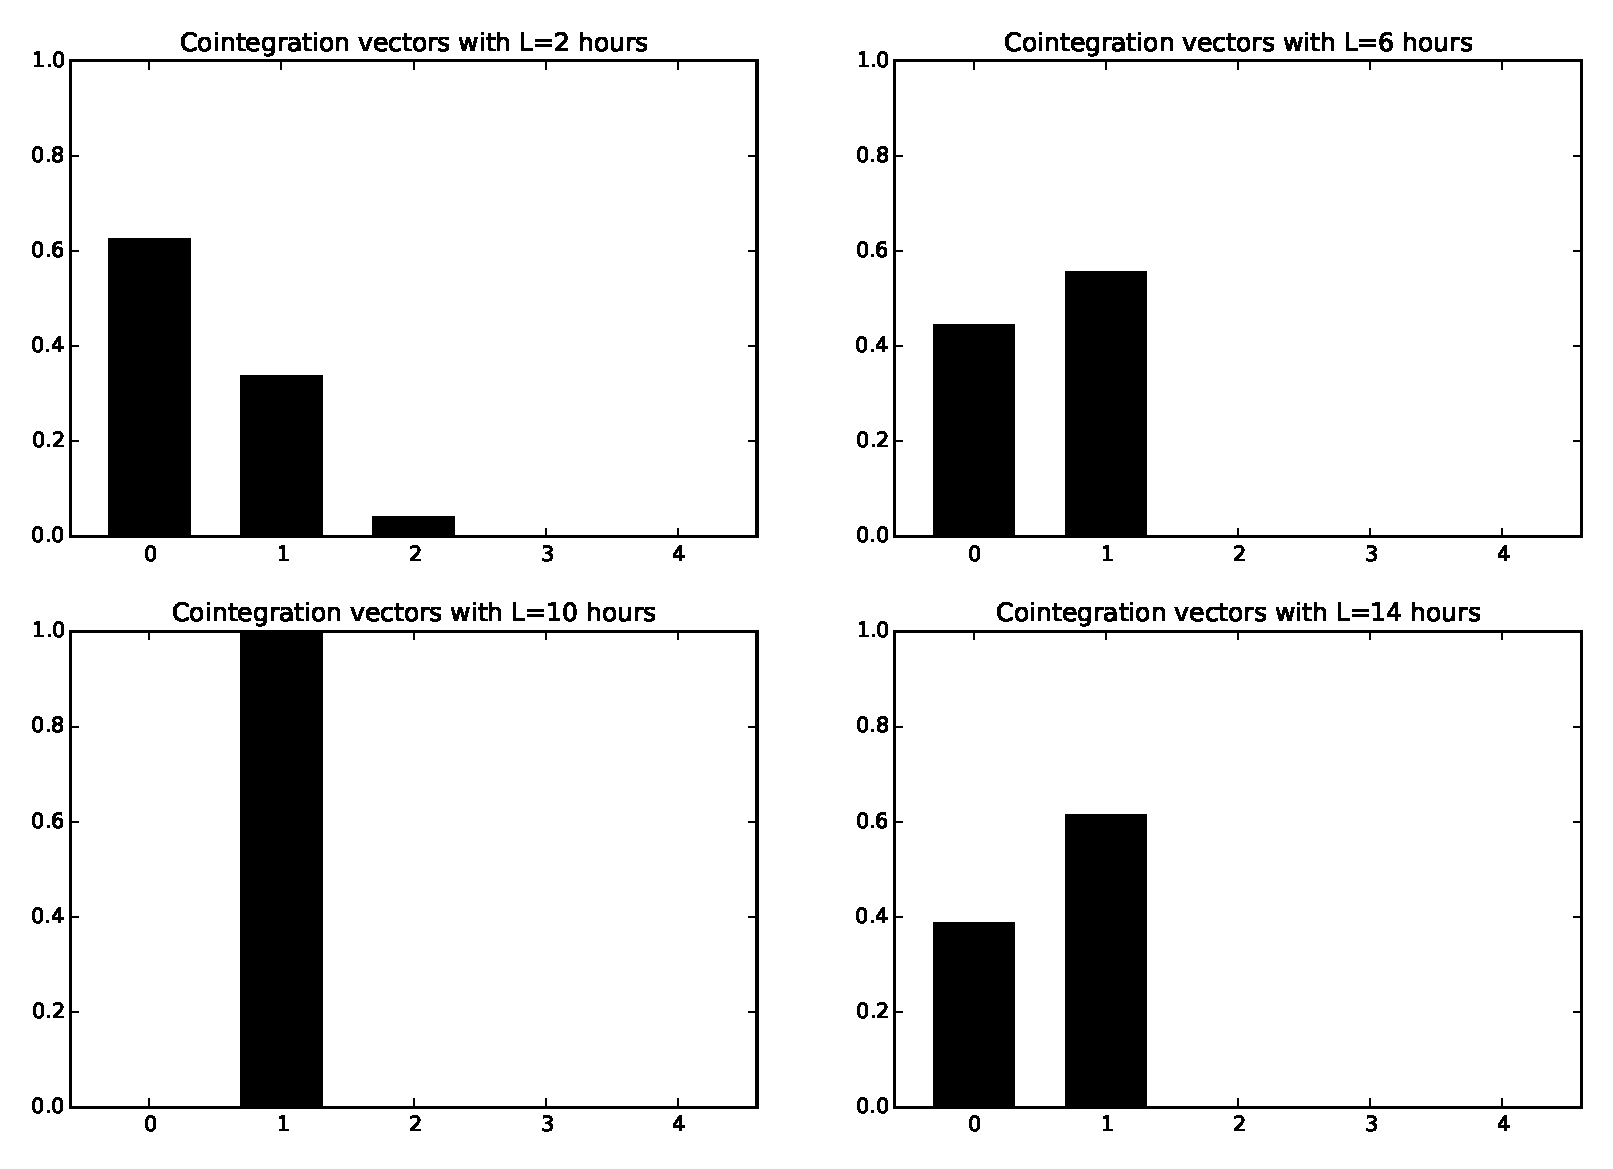
\includegraphics[width=0.9\textwidth]{Fig1}
  \caption{Distribution of the number of cointegration vectors using $p=1$ lags.
  Four possible values for windows size $L$ are shown (2, 6, 10 and 14) hours (1
  hour = 360 data points).}
  \label{fig:hists}
\end{figure}


From section \ref{sec:background} we know that $r=0$ means no cointegration and
$r=l$ (we are using four rates, so $l=4$) reveals that no process is I(1) but
stationary.  The interesting cases of cointegration are those where $r$ lies
strictly between $0$ and $4$, i.e. $0<r<4$.

In order to measure the extent of cointegration, we introduce a
{\em percentage of cointegration\/} as following:
\begin{equation} \label{eq:pcoint}
PC = 
\frac{\#\{ it \mid \text{$it$ has $r$ c.v. with $0<r<l$}\}}
     {\#it}\times 100
\end{equation}
where c.v. stands for cointegration vectors and $it$ is the number of iterations.

The goal of our next experiment was to find a relation between this ratio $PC$
and the performance measure MSE (see equation \ref{eq:MSE}). $L$ was defined
between $[700,1500]$ data points with step size 100 and $p$ took values between
$[1,5]$ with step size 1.  

\begin{figure}[ht!]
  \centering
  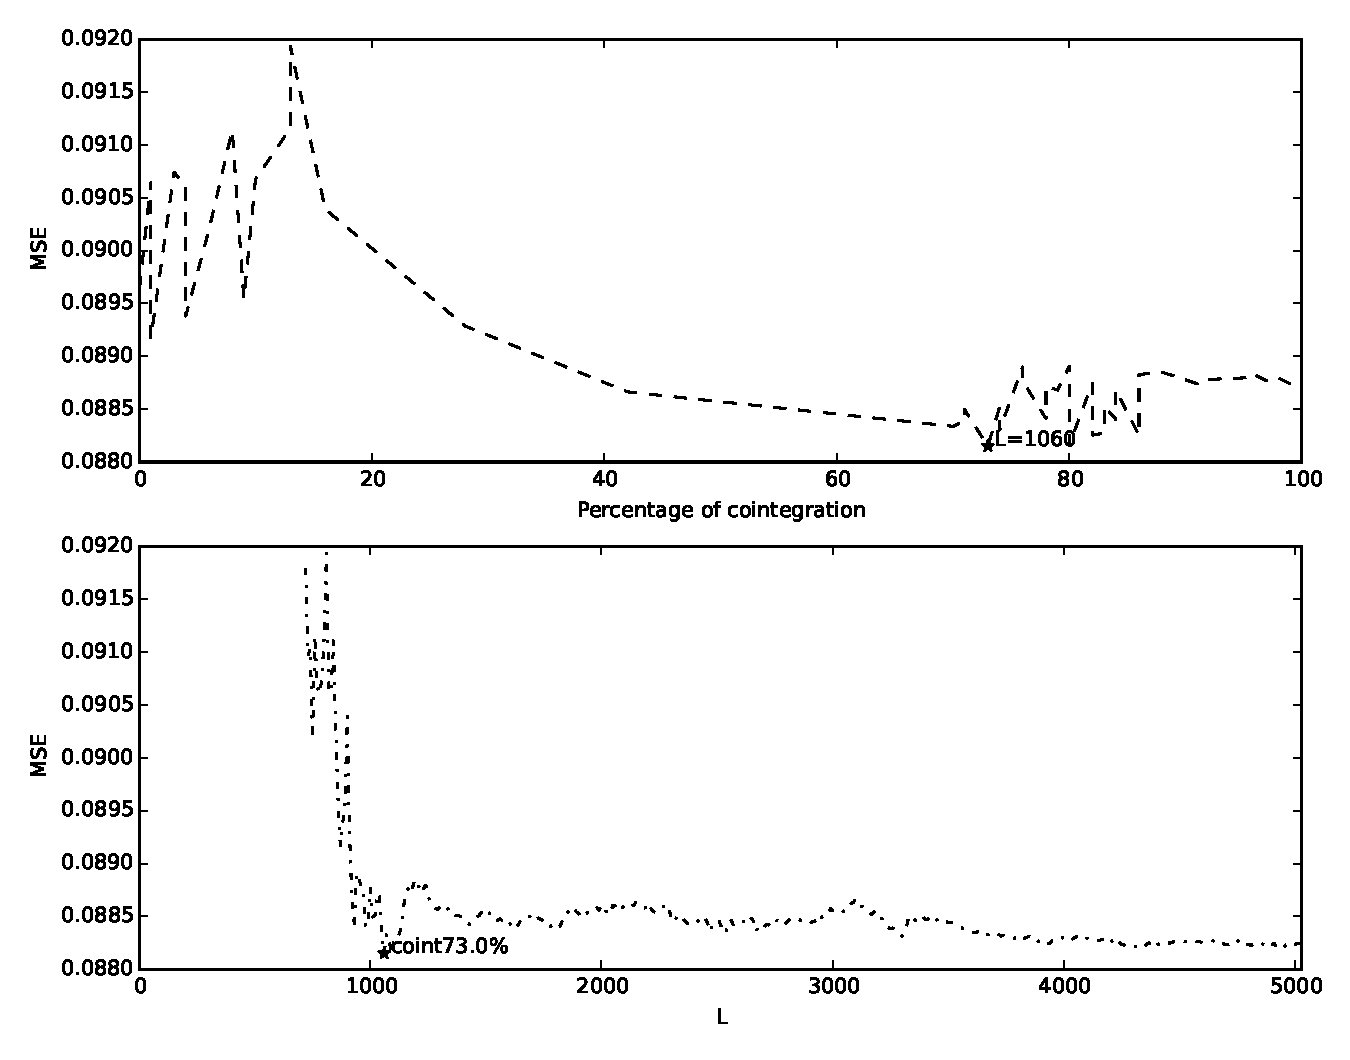
\includegraphics[width=0.9\textwidth]{Fig2}
  \caption{MSE versus the percentage of cointegration considering 1000
  iterations. Best windows size $L$ found was 1060. Below MSE versus $L$ shows a
  rapidly decreasing behaviour, founding minimum at PC = 80\% }
  \label{fig:cointvsmse}
\end{figure}

Figure~\ref{fig:cointvsmse} shows the relation between MSE and $PC$ and $L$.  We
found that better cointegration percentage leads to better performance accuracy
in terms of reducing MSE.

Therefore we proposed to choose $L$ and $p$ in order to maximise the percentage
of cointegration $PC$ in the near past. This process was done every time that
new data was processed. However, this search can be slow if we try different
values for $L$ and $p$ and therefore we distributed this calculation in order to
reduce searching time.

Our proposal is then a modified version of VECM, with parameter $p$ and the
amount of historical data used $L$ obtained at every step. Only the search of
$L$ and $p$ was done in a distributed environment, since this is the most
expensive routine. Our proposal is called Adaptive Vector Error Correction model
(AVECM). AVECM is detailed in the algorithm \ref{alg:AVECM} which summarises
our proposal.

\begin{algorithm}[ht!]
\begin{algorithmic}[1]
\REQUIRE $\,$ \\
$\mathbf{y}$: matrix with $N$ input vectors and $l$ time series\\
$j$: Starting point of testing \\
$it$: Ending point of testing \\
$ps$: list of $p$ values \\
$Ls$: list of $L$ values ($L<N$) \\
$m$: Iterations to determine parameters ($m < N-L$)\\
\ENSURE  $\,$ \\
$\{ \hat{\mathbf{y}}[1],\dots,\hat{\mathbf{y}}[it]\}$: prediction vectors \\
\FOR { $i =j$ to $it$ }
   \STATE $\mathbf{Y} \gets \mathbf{y}[:,i-1]$
    \STATE $L,p \gets
    \texttt{get\_best\_params}(Ls,ps,m,\mathbf{Y})$
        \STATE $model = \text{VECM}(\mathbf{Y},L, p)$
        \STATE $\hat{\mathbf{y}}[i-j] = model.predict()$
\ENDFOR
\end{algorithmic}
\caption{AVECM: Adaptive VECM.}
\label{alg:AVECM}
\end{algorithm}

The input of AVECM is time series prices which are cointegrated. The starting
point of testing is $j$ and the total number of iterations is $it$. We need to
ensure that $j$ is at least the maximum value of $Ls$. $Ls$ and $ps$ are the
possible values for $L$ and $p$.  The function {\bf get\_best\_params} makes
this grid search on the two vector lists $Ls$ and $ps$ and returns the
parameters $L$ and $p$ which maximise the percentage of cointegration $PC$ (see
equation~\ref{eq:pcoint}) for a pre-defined number of iterations $m$. This
function is implemented in a distributed environment, thus ensuring a response
before new data is available.  After $L$ and $p$ parameters are found, VECM is
built and used to forecast the next data point.


\subsection{Model comparison} \label{sec:random}
We compared our proposal, in terms of performance, with the naive forecast of
the random walk model and ARIMA. It is still difficult to outperform the random
walk model for standard econometric forecasting models  despite its
simplicity, see \cite{lo2011}. The random walk model is defined as:

\begin{equation}
\mathbf{y}_t = \mathbf{y}_{t-1} + \epsilon_{t}
\label{rwmodel}
\end{equation}

The naive forecast of the time series difference $\hat{\mathbf{y}}_{t+1}$ for
the random walk model is defined as:
\begin{equation}
\hat{\mathbf{y}}_{t+1} = \mathbf{y}_t + \hat{\epsilon}_{t+1} 
\end{equation}
\noindent where  $\hat{\epsilon}_{t+1} = \epsilon_{t}$.

On the other hand, ARIMA is widely used to forecast returns in finance, see
\cite{tsay2005}. A process can be modelled as an ARIMA$(p,d,q)$ model if
$\mathbf{x}_t=\Delta^d \mathbf{y}_t $, i.e after differencing $d$ times the time
series $\mathbf{y}_t$,  we get an ARMA$(p,q)$. Since we are modelling returns,
we used $d=1$.


\subsection{Evaluation methods} \label{sec:evaluation}

Forecast performance was evaluated using two different methods which are
frequently used in finance:
\begin{description}
\item
{\bf MSE},  Mean Square Error measures the distance between forecasts
and the true values and large deviations from the true value have a
large impact due to squaring forecast error.
\begin{equation}\label{eq:MSE}
\text{MSE} = 
\frac{\displaystyle \sum_{t=1}^{N} (\mathbf{y}_t-\hat{\mathbf{y}}_t)^2}{N}
\end{equation}
\item {\bf $U$-statistic}, the Theil's $U$-statistic, presented by
\cite{theil1966}, is a unit free measure obtained as the ratio between the root
MSE (RMSE) of a model and the RMSE of the naive random walk model. A
$U$-statistic less than 1 implies the performance is better than the naive
model.
\end{description}

\section{\uppercase{Results}}
\label{sec:results}
\noindent The forex market is a 24 hours market which main activity is
dominated by three major trading centers: Tokyo, London and New York. The seven
most important exchange rates are: the Australian Dollar (AUD), the Canadian
Dollar (CAD), the Swiss Franc (CHF), the British Pound Sterling (GBP),the Euro
(EUR), the Japanese Yen (JPY) and the Swedish Krona (SEK)~\cite{HaugetAl2000}.
Most HFT trades are done in those currencies, but increasingly New Zeland (NZD)
and Mexican Peso (MXN) have being automated traded.

Tests of OVECM were carried out using some of the main foreign exchange rates:
EURUSD, GBPUSD, USDCHF, USDJPY ~\cite{Dukascopy2014}. The reciprocal of the last
two rates (CHFUSD, JPYUSD) were used in order to obtain the same base currency
for all rates.  The tests were done using 1-minute frequency data from ask
prices which corresponded to 373.503 data points excluding flat weekends and
holidays from the 12th of August 2013 to the 12th of August 2014.

In estimating the VECM, we firstly checked for unit roots performing the
Augmented Dickey Fuller (ADF) test on the variables in levels and first
differences.

Table~\ref{tab:adf} shows that all currency rates cannot reject the unit root
test but they rejected it with their first differences. This means that all of
them are I(1) time series and we are allowed to use VECM and OVECM.


\begin{table}[h!]
\caption{Unit roots tests}
\label{tab:adf}
\begin{center}
\begin{tabular}{|l|c|c|c|c|c|}
\hline
& \textbf{Statistic} & \textbf{Critical value} & \textbf{Result}\\
\hline
EURUSD          & -0.64 & -1.94 & True       \\
$\Delta$ EURUSD & -70.45   & -1.94 & False       \\
GBPUSD          & -0.63   & -1.94 & True          \\
$\Delta$ GBPUSD & -54.53   & -1.94 & False       \\
CHFUSD          & -0.88   & -1.94 & True         \\
$\Delta$ CHFUSD & -98.98   & -1.94 & False       \\
JPYUSD          & -0.65 & -1.94 & True        \\
$\Delta$ JPYUSD & -85.78 & -1.94 & False     \\ 
\hline
\end{tabular}
\end{center}
\end{table}


\subsection{Setting parameters}

In order to set VECM parameter: $L$ and $p$, we use the Akaike Information
Criterion (AIC). RR parameter $\lambda$ was done by cross-validation.

\begin{figure}[h!]
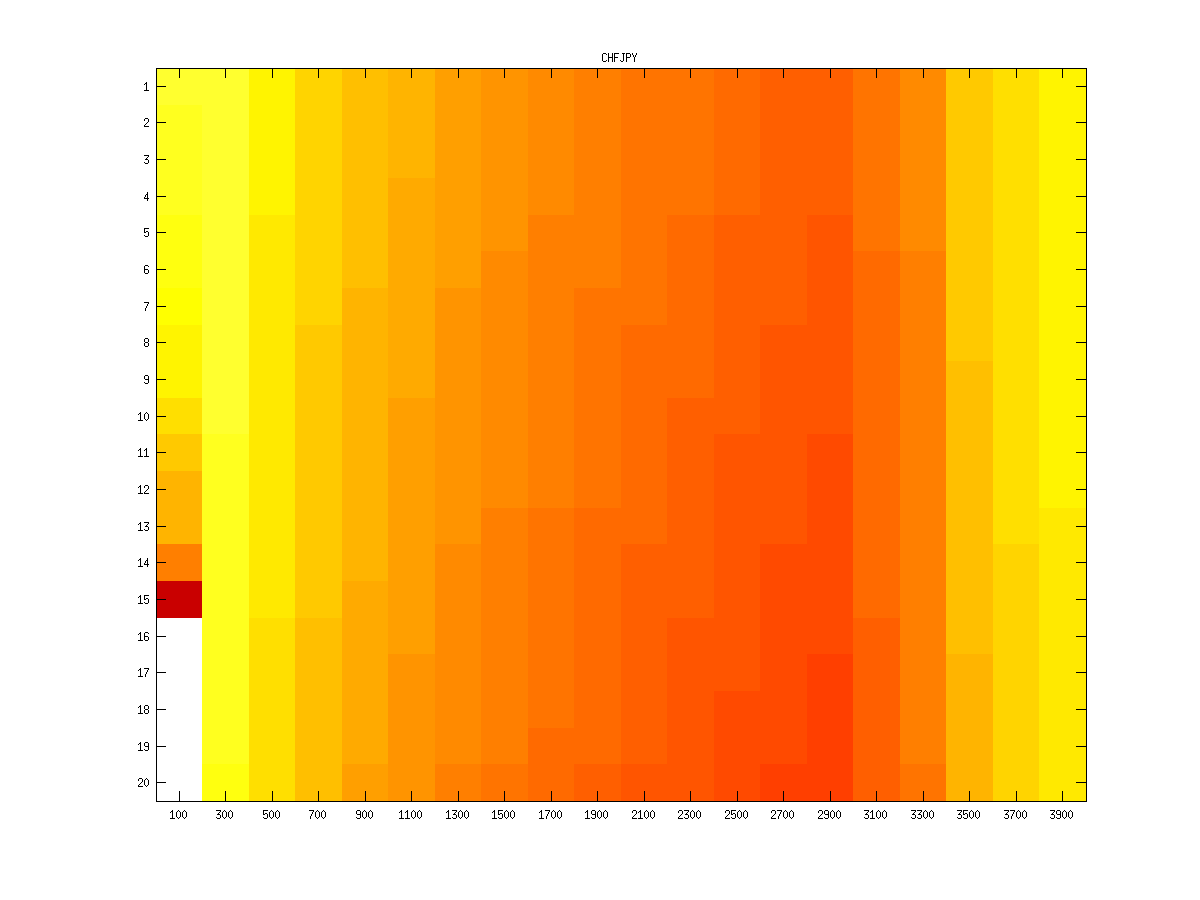
\includegraphics[width=0.5\linewidth]{img/vecm-params}
\caption{Setting VECM parameters}
\label{fig:shrinks}
\end{figure}

We ran OVECM and SLVECM 10.000 iterations for different values of sliding
window size $L$, number of lags $p$ and mean\_error (the latest only appliesto
OVECM). The execution times are shown in the table~\ref{tab:extimes}.

\begin{table}[h!]
\caption{Execution times}
\label{tab:extimes}
\begin{center}
\begin{tabular}{|l|c|c|c|c|c|}
\hline
& \textbf{L} & \textbf{P} & \textbf{mean\_error}  & \textbf{Time} \\
\hline
SLVECM & 300 & 4  & -- & 144\\
OVECM & 300 & 4  & 0 & 98\\
OVECM & 300 & 4  & 120 & 78\\
\hline
SLVECM & 300 & 8  & -- & 298\\
OVECM & 300 & 8  & 0 & 196\\
OVECM & 300 & 8  & 120 & 177\\
\hline
SLVECM & 3000 & 4  & -- & 324\\
OVECM & 3000 & 4  & 0 & 241\\
OVECM & 3000 & 4  & 120 & 97\\
\hline
SLVECM & 3000 & 8  & -- & 860\\
OVECM & 3000 & 8  & 0 & 632\\
OVECM & 3000 & 8  & 120 & 303\\
\hline
\end{tabular}
\end{center}
\end{table}

It is clear that execution time depends directly on $L$ and $p$ since they
determine the size of matrix $\mathbf{A}$ and therefore affect the OLS function
execution time.
It is worthy of note that execution time also depends on mean\_error because it
determines how many times OVECM will recalculate cointegration vectors which is
an expensive routine. Also, our proposal reduces execution time more than  50\%
in some cases.

Figure~\ref{fig:mapes} shows an example of the
in-sample MAPE. In consequence, OVECM performance increases when
mean\_error increases, but it will affect accuracy. Table~\ref{tab:mapes} shows
differents MAPEs out-of-sample for SLVECM and OVECM and all of them are very
similar. This supports the theory that cointegration vectors little with time.

\begin{table*}[ht!]
\caption{Out-of-sample MAPEs}
\label{tab:mapes}
\begin{center}
\begin{tabular}{|l|c|c|c|c|c|c|c|}
\hline
Method & \textbf{L} & \textbf{P} & \textbf{mean}  & \textbf{MAPE} & \textbf{MAPE}& \textbf{MAPE}& \textbf{MAPE}\\
&  &  & \textbf{error}  & \textbf{EURUSD} & \textbf{GBPUSD}& \textbf{CHFUSD}& \textbf{JPYUSD}\\
\hline
 SLVECM &   L=300 &  P=4&    &  134.76&  136.50&  133.16&  137.20\\
 OVECM  &   L=300 &  P=4& 0  &  134.76&  136.50&  133.16&  137.20\\
 OVECM  &   L=300 &  P=4& 120&  134.30&  135.53&  132.88&  136.44\\
\hline
 SLVECM &   L=300 &  P=8&    &  157.76&  160.55&  155.24&  162.74\\
 OVECM  &   L=300 &  P=8& 0  &  157.76&  160.55&  155.24&  162.74\\
 OVECM  &   L=300 &  P=8& 120&  158.03&  160.89&  155.30&  162.61\\
\hline
 SLVECM &   L=3000&  P=4&    &  111.91&  110.60&  109.22&  105.69\\
 OVECM  &   L=3000&  P=4& 0  &  111.91&  110.60&  109.22&  105.69\\
 OVECM  &   L=3000&  P=4& 120&  112.49&  111.26&  109.25&  105.88\\
\hline
 SLVECM &   L=3000&  P=8&    &  118.96&  118.97&  114.99&  110.57\\
 OVECM  &   L=3000&  P=8& 0  &  118.96&  118.97&  114.99&  110.57\\
 OVECM  &   L=3000&  P=8& 120&  119.23&  119.05&  114.82&  110.58\\
\hline
\end{tabular}
\end{center}
\end{table*}


% SLVECM    L=300   P=4             [ 134.7630329035  136.5086625175  133.1658744763  137.2084992162]
% SLVECM    L=300   P=8             [ 157.761485001   160.5552885679  155.2402883372  162.7438222296]
% SLVECM    L=3000  P=4             [ 111.91007246    110.6026357988  109.2219354574  105.6932468374]
% SLVECM    L=3000  P=8             [ 118.9663817354  118.9770962212  114.9939599829  110.5712975915]
% OVECM     L=300   P=4 AVGE=0      [ 134.7630329035  136.5086625175  133.1658744763  137.2084992162]
% OVECM     L=300   P=8 AVGE=0      [ 157.761485001   160.5552885679  155.2402883372  162.7438222296]
% OVECM     L=3000  P=4 AVGE=0      [ 111.91007246    110.6026357988  109.2219354574  105.6932468374]
% OVECM     L=3000  P=8 AVGE=0      [ 118.9663817354  118.9770962212  114.9939599829  110.5712975915]
% OVECM     L=300   P=4 AVGE=120    [ 134.301881303   135.5315795893  132.8835616177  136.4493817757]
% OVECM     L=300   P=8 AVGE=120    [ 158.0383643503  160.8908753314  155.3006014391  162.6119716451]
% OVECM     L=3000  P=4 AVGE=120    [ 112.4957023005  111.2666209761  109.2525274819  105.8804205046]
% OVECM     L=3000  P=8 AVGE=120    [ 119.2383924719  119.0508650247  114.8288372278  110.5815700448]


%\begin{figure}[!h]
%  \vspace{-0.2cm}
%  \centering
%   {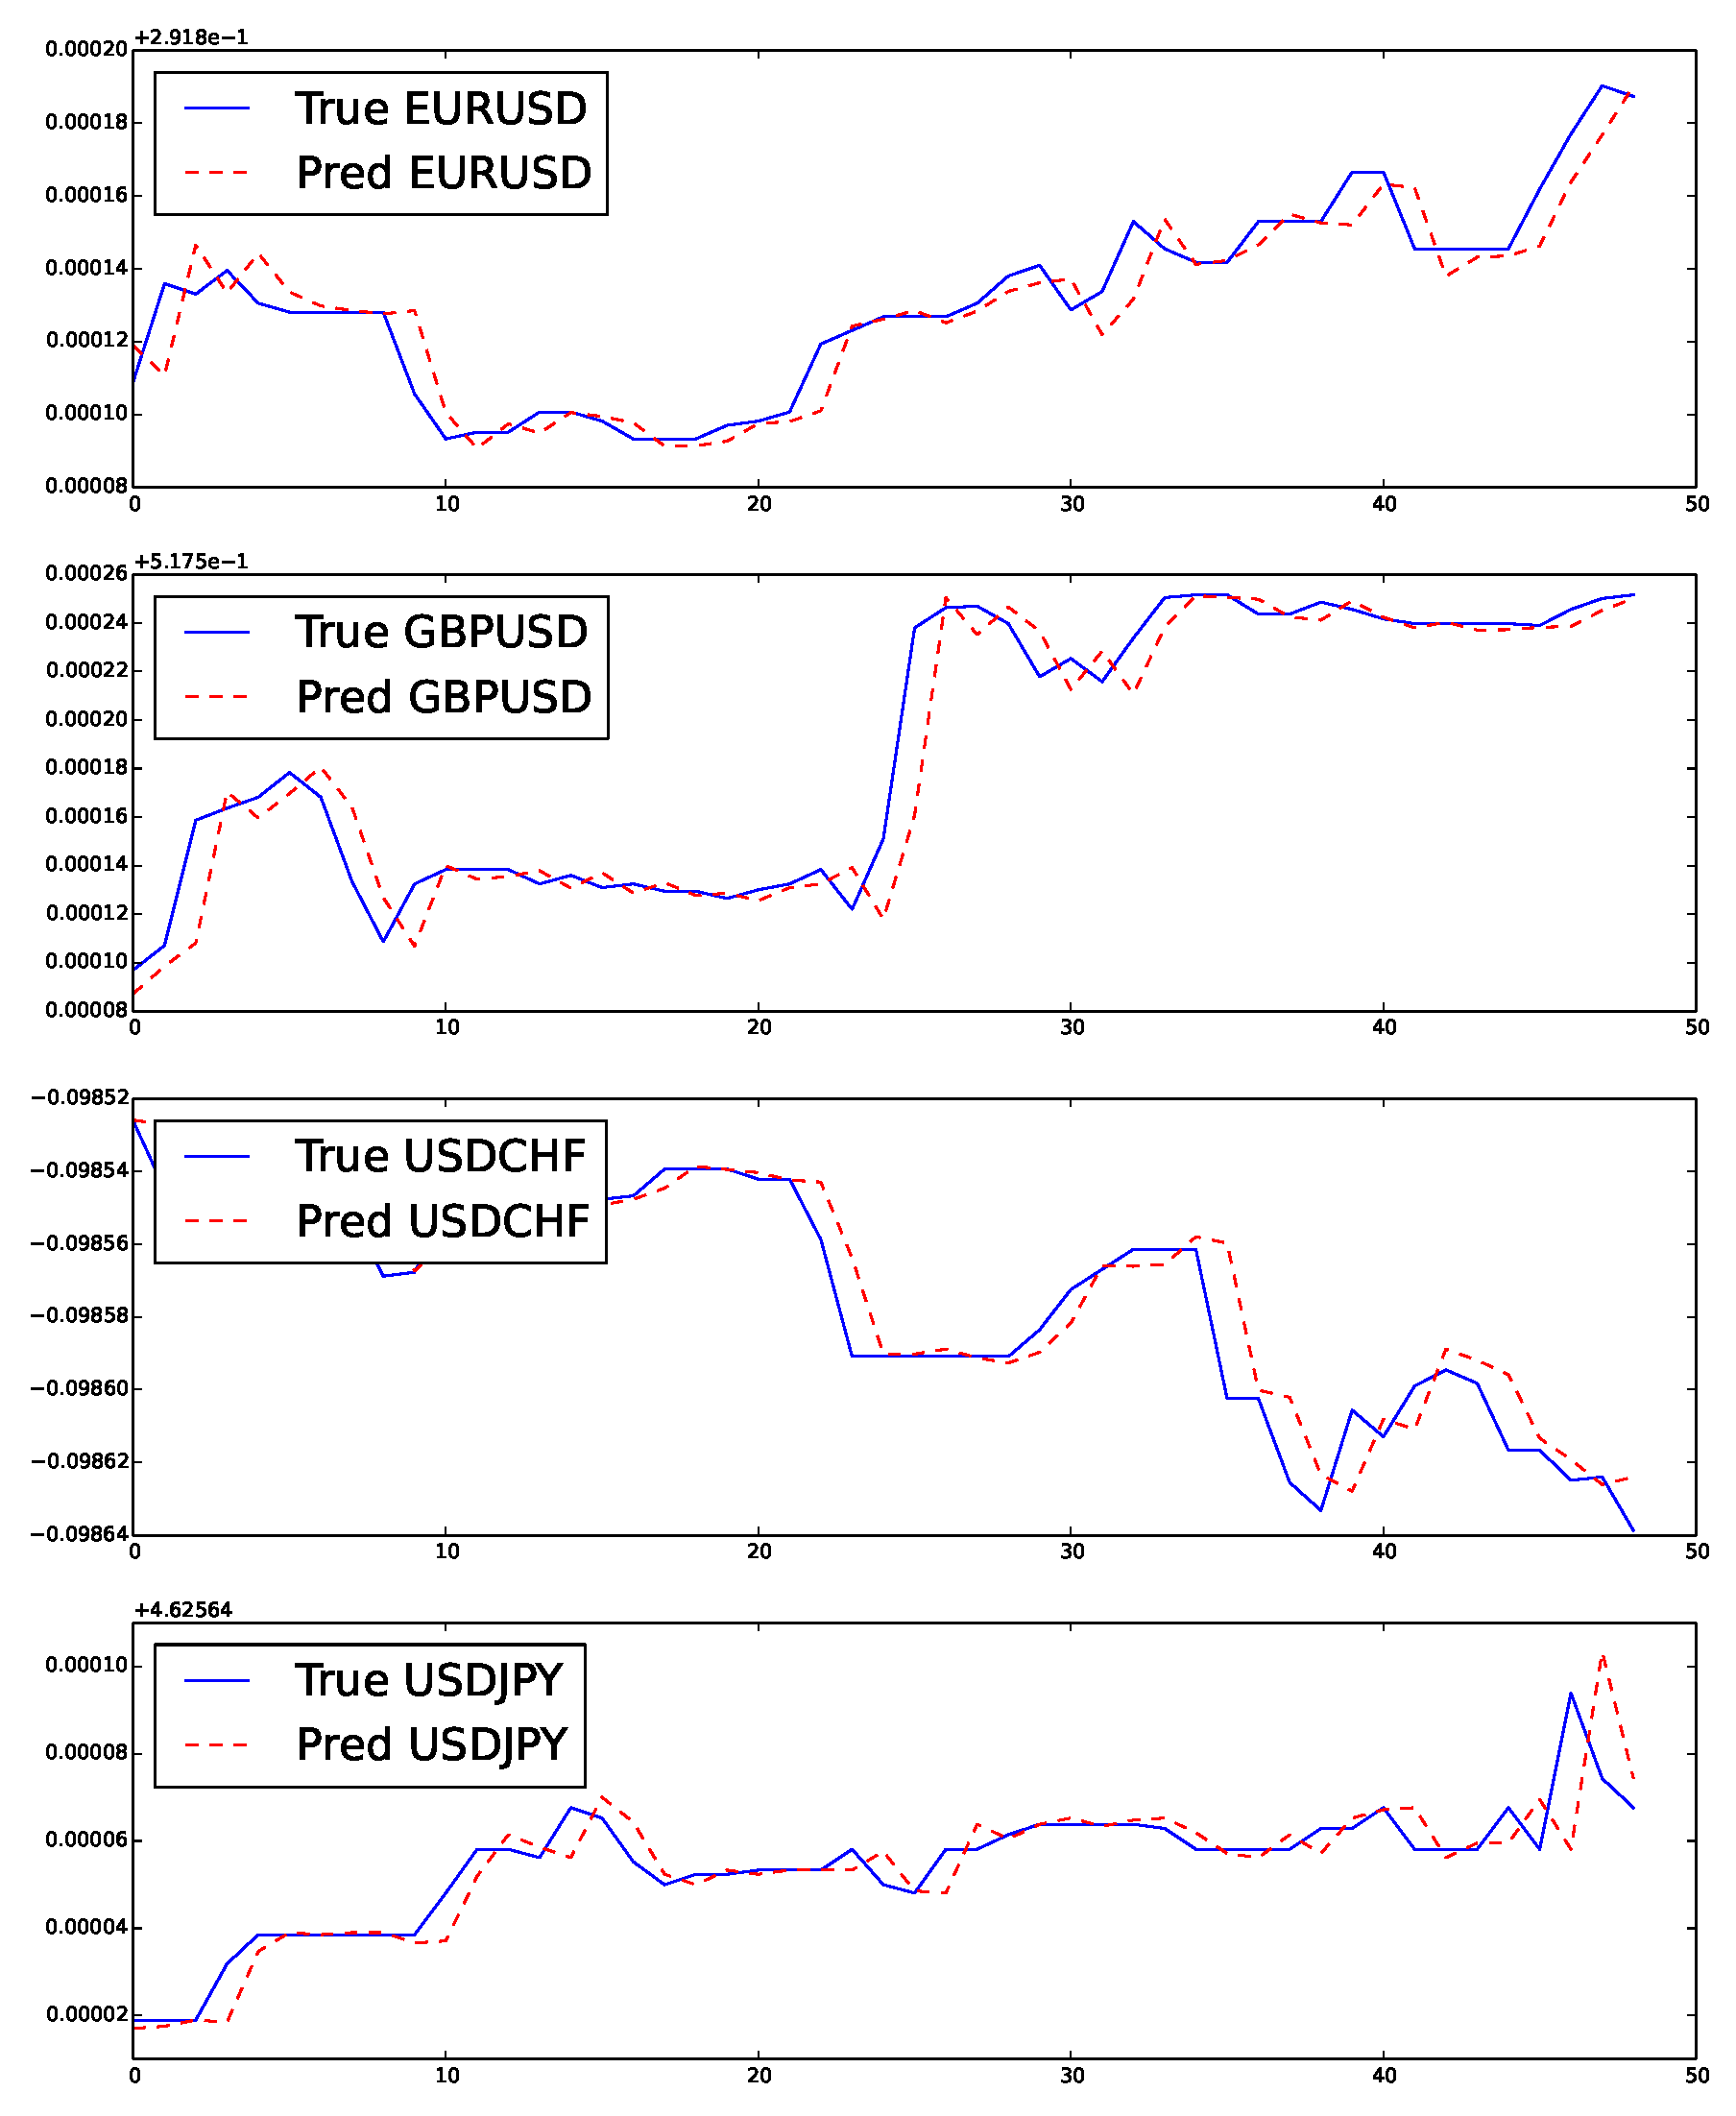
\epsfig{file = img/accuracy.eps, width = 7.5cm}}
%  \caption{Time series differences accuracy.}
%  \label{fig:accuracy}
% \end{figure}
%
%\begin{figure}[!h]
%  \vspace{-0.2cm}
%  \centering
%   {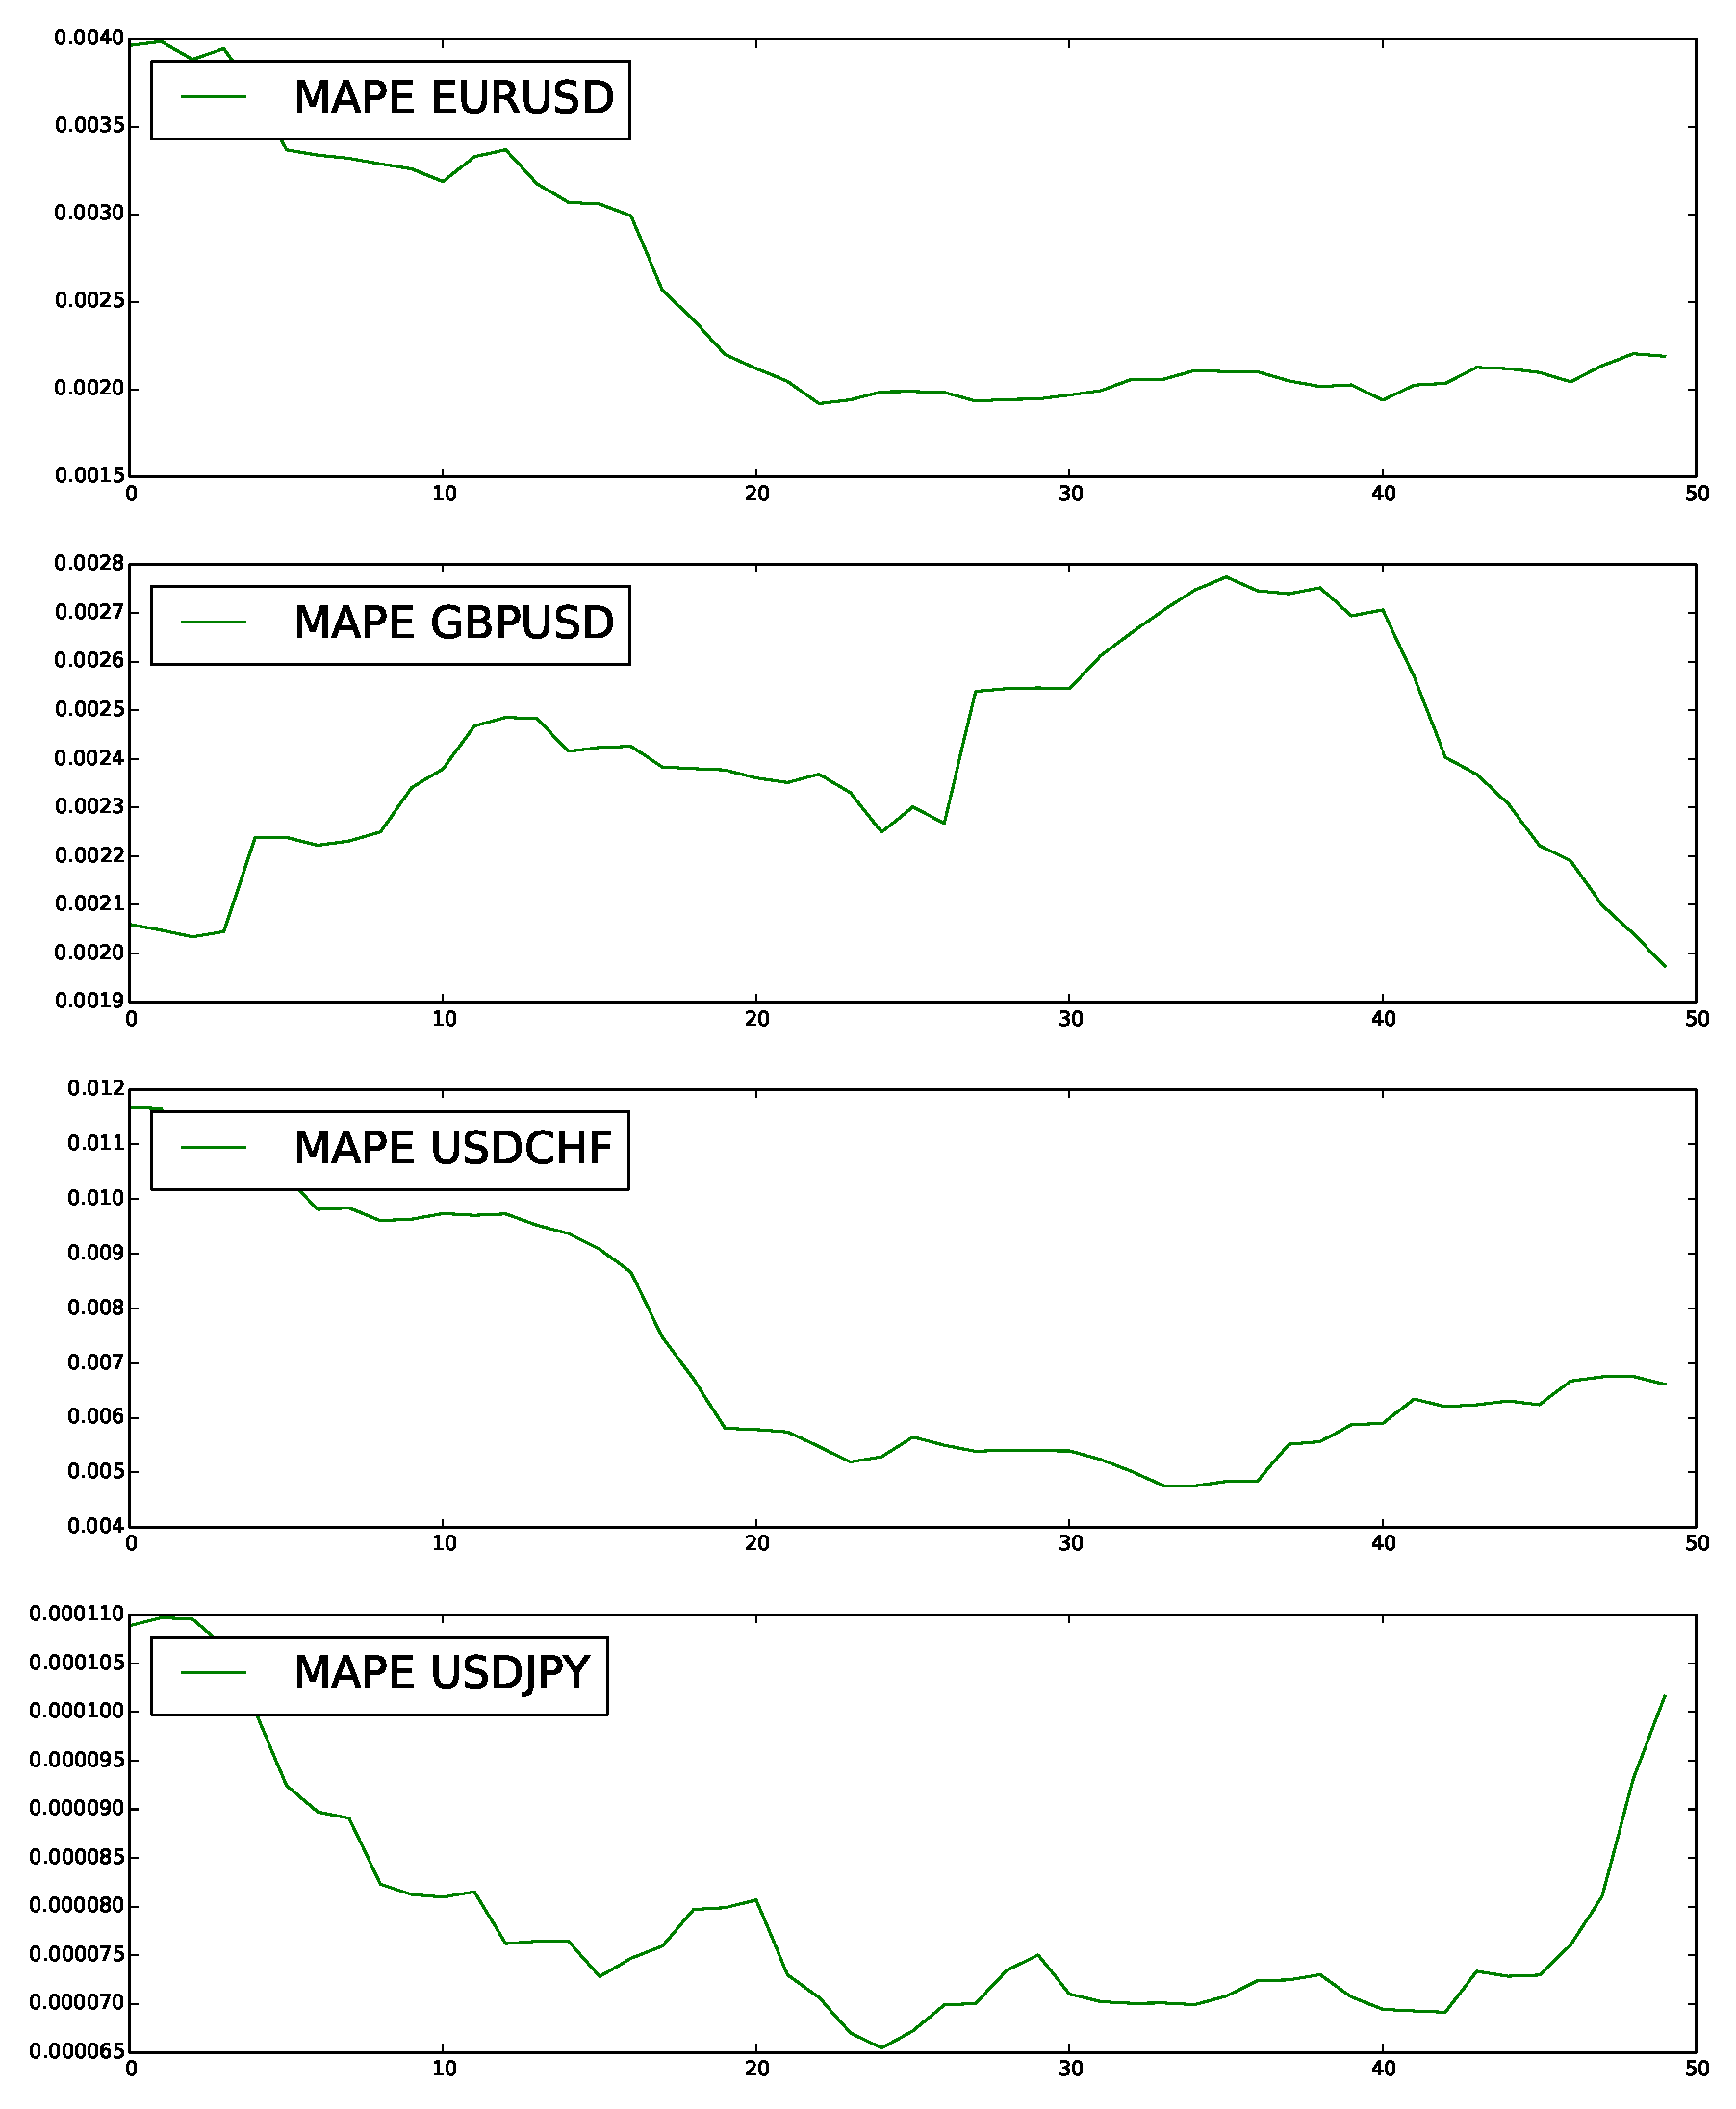
\epsfig{file = img/mapes.eps, width = 7.5cm}}
%  \caption{In-sample MAPEs example.}
%  \label{fig:mapes}
% \end{figure}

Despite the fact that MAPEs are high, figure ~\ref{fig:accuracy} shows some of
the out-of-sample forecasts made by our proposal OVECM which appears to follow
time series differences. 


\section{Conclusion} \label{sec:conclusion}

Conclusions here

\bibliographystyle{apalike}
\bibliography{reference}
%\begin{thebibliography}{9}
%
%\bibitem{smola}
%Bernhard Scholkopf and Alexander J. Smola. 
%\emph{Learning with Kernels: Support Vector Machines, 
%Regularization, Optimization, and Beyond.}.
%MIT Press, Cambridge, MA, USA, 2001
%
%\bibitem{wiki}
%\url{http://en.wikipedia.org/wiki/Reproducing_kernel_Hilbert_space}
%
%\bibitem{wikibooksIsom}
%\url{http://en.wikibooks.org/wiki/Linear_Algebra/Definition_and_Examples_of_Isomorphisms}
%
%\bibitem{wolframREq}
%\url{http://mathworld.wolfram.com/EquivalenceRelation.html}
%
%\bibitem{wikiHomoM}
%\url{http://en.wikipedia.org/wiki/Homomorphism}
%
%
%\end{thebibliography}

\end{document}
